\documentclass[11pt]{article}

\usepackage[T1]{fontenc}
\usepackage{lmodern}
\usepackage[a4paper,margin=2.4cm]{geometry}
\usepackage{amsmath,amssymb,amsthm,mathtools}
\usepackage{graphicx}
\usepackage{booktabs,tabularx,array,longtable}
\usepackage{enumitem}
\usepackage{framed}
\usepackage{float}
\usepackage[dvipsnames,svgnames]{xcolor}
\usepackage{tikz}
\usetikzlibrary{arrows.meta,positioning,shapes.geometric,shapes.misc,fit,backgrounds,calc,decorations.pathreplacing}
\usepackage[colorlinks=true,linkcolor=NavyBlue,citecolor=NavyBlue,urlcolor=NavyBlue]{hyperref}

% ---------------------------------------------------------------- theorems
\theoremstyle{plain}
\newtheorem{proposition}{Proposition}[section]
\newtheorem{lemma}[proposition]{Lemma}
\theoremstyle{definition}
\newtheorem{definition}[proposition]{Definition}
\newtheorem{example}[proposition]{Example}
\theoremstyle{remark}
\newtheorem{remark}[proposition]{Remark}

% ---------------------------------------------------------------- notation
\newcommand{\peb}[2]{\ensuremath{\langle #1,\,#2\rangle}}   % pebble
\newcommand{\rk}{\operatorname{rk}}                          % rank in a sort
\newcommand{\Hard}{\mathcal{H}}                              % hard pebbles
\newcommand{\Need}{N}                                        % needs
\newcommand{\Adm}{\mathrm{Adm}}                              % admissible slots
\newcommand{\Slots}{\mathcal{S}}
\newcommand{\Travs}{\mathcal{T}}
\newcommand{\code}[1]{\nolinkurl{#1}}
\newcommand{\file}[1]{{\small\nolinkurl{#1}}}

% ---------------------------------------------------------------- colours
\definecolor{cslot}{HTML}{2F6DB5}    % slots / positions
\definecolor{ctrav}{HTML}{D9822B}    % travs / identities
\definecolor{cold}{HTML}{8E44AD}     % old greedy fill
\definecolor{cnew}{HTML}{2E8B57}     % new monotone matching
\definecolor{cbad}{HTML}{C0392B}     % losses, failures
\definecolor{cgrey}{HTML}{8A8F98}
\definecolor{clight}{HTML}{EEF2F7}
\definecolor{cbox}{HTML}{F6F8FB}

% ---------------------------------------------------------------- boxes
\newenvironment{keybox}[1]{%
  \def\FrameCommand{\fboxsep=8pt\fcolorbox{cslot!60}{cbox}}%
  \MakeFramed{\advance\hsize-\width \FrameRestore}%
  \noindent\textbf{\color{cslot}#1}\par\smallskip}%
  {\endMakeFramed}

\newenvironment{factbox}{%
  \def\FrameCommand{\fboxsep=6pt\fcolorbox{cgrey!50}{white}}%
  \MakeFramed{\advance\hsize-\width \FrameRestore}\small}%
  {\endMakeFramed}

% ---------------------------------------------------------------- tikz styles
\tikzset{
  box/.style={draw, rounded corners=2pt, minimum height=6mm, inner sep=3pt, font=\small, fill=white, align=center},
  slotn/.style={box, fill=cslot!12, draw=cslot},
  travn/.style={box, fill=ctrav!15, draw=ctrav},
  plain/.style={box, draw=cgrey, text=black!80},
  oldn/.style={box, fill=cold!10, draw=cold},
  newn/.style={box, fill=cnew!10, draw=cnew},
  badn/.style={box, fill=cbad!10, draw=cbad},
  dec/.style={box, diamond, aspect=2.4, inner sep=1pt, fill=white},
  conn/.style={circle, draw, fill=white, inner sep=0pt, minimum size=3.2mm},
  pre/.style={-{Stealth[length=2.2mm]}, thick},
  thinpre/.style={-{Stealth[length=1.8mm]}},
  cut/.style={pre, draw=cnew, densely dashed},
  back/.style={pre, draw=ctrav, dashed},
  bad/.style={pre, draw=cbad},
  pebble/.style={circle, draw, fill=white, inner sep=0pt, minimum size=4.4mm, font=\scriptsize},
  spebble/.style={pebble, fill=cslot!70, draw=cslot!90!black, text=white},
  tpebble/.style={pebble, fill=ctrav!80, draw=ctrav!90!black, text=white},
  ghost/.style={pebble, dashed, draw=cgrey, text=cgrey},
  lbl/.style={font=\scriptsize, text=black!70},
  note/.style={font=\scriptsize\itshape, text=black!65, align=left},
}

\emergencystretch=2.5em
\urlstyle{tt}
\def\UrlBreaks{\do\/\do\_\do\-\do\.\do\,\do\(\do\)\do\:}
\Urlmuskip=0mu plus 1mu
\mathchardef\UrlBreakPenalty=100
\setlist{itemsep=2pt, topsep=4pt}
\newcolumntype{L}{>{\raggedright\arraybackslash}X}

\title{From greedy fill to monotone matching\\[4pt]
\large How first pass chooses item identities, then and now}
\author{Explainer for exfret's property randomizer (\texttt{propertyrandomizer})}
\date{26 September 2026}

\begin{document}
\maketitle

\section*{Summary}
\addcontentsline{toc}{section}{Summary}

\begin{keybox}{Short answer: a new algorithm for the same problem}
The \emph{problem} first pass solves hasn't changed. It still splits each item into a \emph{position} (slot) and an \emph{identity} (trav) and picks a one-to-one assignment of identities to positions of the same type, within a cost window. Item reflection then turns that assignment into the game, and promotion reasons over the same split graph.

The \emph{search} that picks the assignment is new. None of the greedy fill's machinery survived: its reachability tests, reservations, target mechanic, swap chains and ``desperation'' mode are all gone.
\begin{itemize}
  \item \textbf{Old (greedy forward fill):} built the assignment one pair at a time, in the order of an imagined playthrough, starting from nothing. When it got stuck, the attempt failed.
  \item \textbf{New (monotone matching):} starts from the vanilla assignment, which is valid by definition. It then replaces the \emph{whole} assignment three times, each time with a random one that keeps every protected context. When a proposal fails the check and can't be repaired, it keeps the assignment it already had.
\end{itemize}
It's new in a second sense too. First pass now reasons the way promotion does, with pebbles, ranks, backings that go strictly earlier, and a fallback that's always available. So unified randomization rests on one theory instead of two.
\end{keybox}

\medskip
\noindent The four changes that matter:

\begin{enumerate}[leftmargin=*]
  \item \textbf{From building to moving.} The greedy fill grew a partial assignment and could reach a dead end. Monotone matching always holds a complete, valid assignment and moves from one valid assignment to another (Proposition~\ref{prop:invariant}).
  \item \textbf{From ``reachable'' to ``reachable in the right contexts''.} The greedy asked whether a slot or identity had \emph{some} context. The new first pass asks, for each protected pebble (node, room, abilities), whether it's still there, and checks that exactly with a fresh sort (the \emph{gate}).
  \item \textbf{From reservations to proofs.} The greedy steered by holding back identities that didn't help the next mechanic on the science-pack path. The new first pass proves every protected pebble in a random sort and pins an identity only in the contexts where the proof uses it. Every other identity may go anywhere its type and cost allow.
  \item \textbf{The rank rule.} A needed identity may only move to a position that, in each context it's needed in, is reached \emph{before} the identity was reached in the current sort. Needed identities therefore only move earlier, which is where the name \emph{monotone} comes from.
\end{enumerate}

\begin{table}[H]
\centering\small
\begin{tabularx}{\textwidth}{@{}p{3.2cm}LL@{}}
\toprule
& \textbf{Greedy forward fill (until 26 Sep)} & \textbf{Monotone matching (now)}\\
\midrule
Starts from & the empty assignment & the vanilla assignment\\
Unit of choice & one slot/identity pair at a time & the whole matching, per round\\
Validity test & slot or identity has \emph{some} context & every hard pebble kept, checked by a fresh sort\\
Steering & reservations toward the next targeted mechanic & needs from proofs, plus the rank rule\\
What's protected & targeted mechanics, by node, once reached anywhere & all protected mechanic pebbles, planet-locked recipes, and every recipe reachable\\
When stuck & retry below 50\%, else turn off the checks & keep the previous matching (always valid)\\
Measured losses & lost isolatable contexts on every measured seed & 0 protected contexts lost by first pass\\
Identities moved & not measured & 237--247 of 255 per round\\
\bottomrule
\end{tabularx}
\caption{At a glance. The greedy's measurements are from the 25 September investigation (Section~\ref{sec:greedy-losses}); the new ones are from 26 September runs (Section~\ref{sec:measure}).}
\label{tab:glance}
\end{table}

\bigskip
{\setcounter{tocdepth}{2}\tableofcontents}
\clearpage
\section{The problem both versions solve}
\label{sec:problem}

First pass runs inside unified randomization (\file{randomizations/graph/unified/execute-new.lua}), before the other handlers. It fixes item randomization's permutation, which says which item \emph{identity} each item \emph{position} gets. The handlers that run after it (promotion, recipe ingredients, and the rest) then reason over the graph first pass built. This section covers what stayed the same from the greedy fill to monotone matching.

\subsection{Positions and identities}

For every node that takes part, first pass splits the logic-graph node into two nodes (\file{first-pass-new.lua}, ``SPLIT GRAPH NODES''):

\begin{description}[leftmargin=1.2em, style=nextline]
  \item[Slot (the position).] It keeps the node's name and the edges that say \emph{where the item comes from} and \emph{which recipes use it}. These are crafting, loot, burnt results, items that spoil into it, resource and asteroid mining, and recipe ingredient uses (the \code{always_slot_pre} and \code{always_slot_dep} tables in \file{compat/vanilla.lua}). Any edge a handler randomizes (a base or head) also stays on the slot.
  \item[Trav (the identity), named \texttt{X-trav}.] It gets every other fixed edge, which says \emph{what the item is}: it places a building, it's a fuel, it's launched and delivered. It also gets sources that follow the item's name. In the model, mining a building or a tile gives the item under its own name (\code{dutils.mining_keeps_item_names}), so that edge belongs to the identity. Entity randomization's identity heads and bases move here too.
\end{description}

\noindent The edge slot $\to$ trav is then cut into a base (on the slot) and a head (on the trav). Choosing the assignment means choosing which base connects to which head. Items get one extra edge, trav $\to$ slot. After reflection, the item made at a position \emph{is} the identity's item, so the position's consumers also get the identity's own sources, such as delivery to other rooms or spoiling (\code{connect} in \file{monotone-matching.lua}).

\begin{figure}[tbp]
\centering
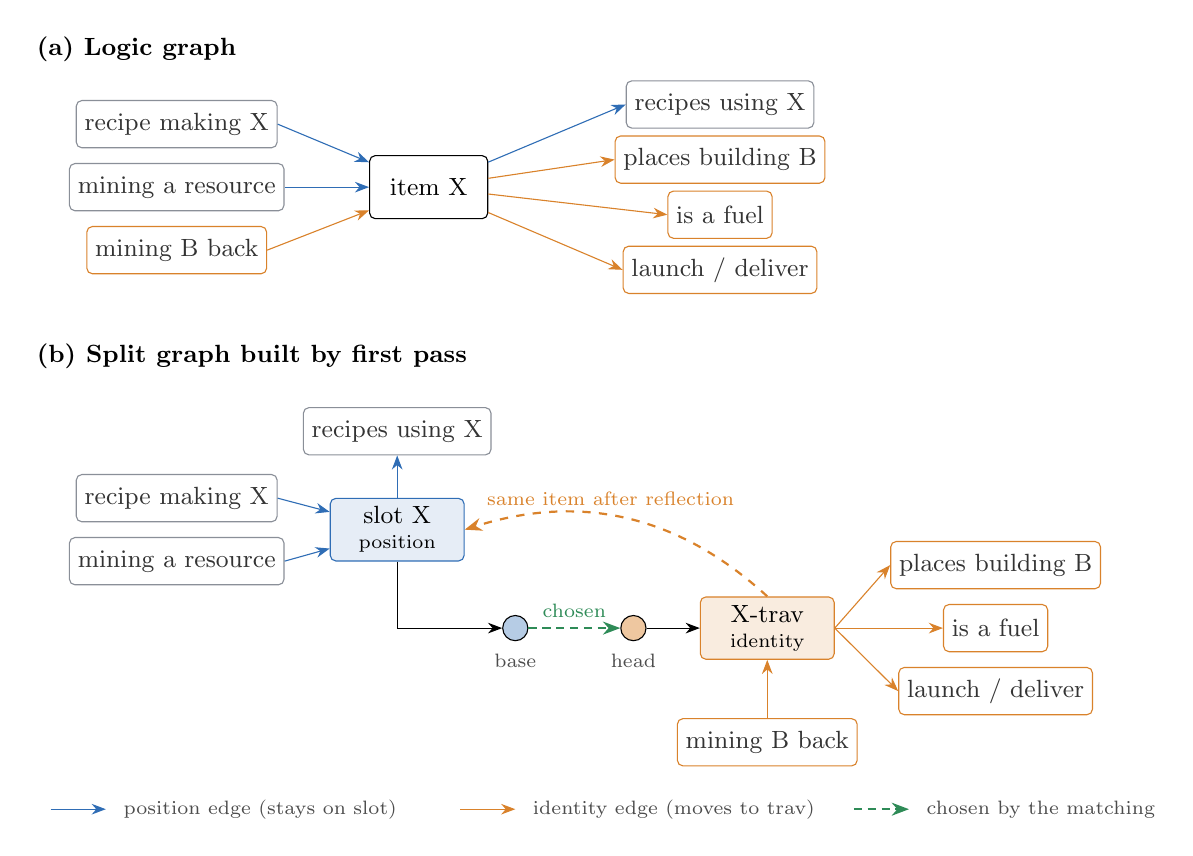
\begin{tikzpicture}[x=1cm,y=1cm]
% ---------------- (a) logic graph
\node[anchor=west, font=\small\bfseries] at (-6.9,1.75) {(a) Logic graph};
\node[plain] (pa1) at (-5.0,0.8) {recipe making X};
\node[plain] (pa2) at (-5.0,0.0) {mining a resource};
\node[plain, draw=ctrav] (pa3) at (-5.0,-0.8) {mining B back};
\node[box, minimum width=1.5cm, minimum height=8mm] (xa) at (-1.8,0) {item X};
\node[plain] (ua1) at (1.9,1.05) {recipes using X};
\node[plain, draw=ctrav] (ua2) at (1.9,0.35) {places building B};
\node[plain, draw=ctrav] (ua3) at (1.9,-0.35) {is a fuel};
\node[plain, draw=ctrav] (ua4) at (1.9,-1.05) {launch / deliver};
\draw[thinpre, draw=cslot] (pa1.east) -- (xa);
\draw[thinpre, draw=cslot] (pa2.east) -- (xa);
\draw[thinpre, draw=ctrav] (pa3.east) -- (xa);
\draw[thinpre, draw=cslot] (xa) -- (ua1.west);
\foreach \u in {ua2,ua3,ua4} \draw[thinpre, draw=ctrav] (xa) -- (\u.west);
% ---------------- (b) split graph
\begin{scope}[yshift=-4.7cm]
\node[anchor=west, font=\small\bfseries] at (-6.9,2.55) {(b) Split graph built by first pass};
\node[plain] (pb1) at (-5.0,0.75) {recipe making X};
\node[plain] (pb2) at (-5.0,-0.05) {mining a resource};
\node[slotn, minimum width=1.7cm] (slot) at (-2.2,0.35) {slot X\\[-2pt]{\scriptsize position}};
\node[plain] (ub1) at (-2.2,1.6) {recipes using X};
\node[conn, fill=cslot!35] (base) at (-0.7,-0.9) {};
\node[conn, fill=ctrav!45] (head) at (0.8,-0.9) {};
\node[lbl, below=1pt of base] {base};
\node[lbl, below=1pt of head] {head};
\node[travn, minimum width=1.7cm] (trav) at (2.5,-0.9) {X-trav\\[-2pt]{\scriptsize identity}};
\node[plain, draw=ctrav] (ub2) at (5.4,-0.1) {places building B};
\node[plain, draw=ctrav] (ub3) at (5.4,-0.9) {is a fuel};
\node[plain, draw=ctrav] (ub4) at (5.4,-1.7) {launch / deliver};
\node[plain, draw=ctrav] (pb3) at (2.5,-2.35) {mining B back};
\draw[thinpre, draw=cslot] (pb1.east) -- (slot);
\draw[thinpre, draw=cslot] (pb2.east) -- (slot);
\draw[thinpre, draw=cslot] (slot.north) -- (ub1.south);
\draw[thinpre] (slot.south) |- (base.west);
\draw[cut] (base) -- node[above, lbl, text=cnew] {chosen} (head);
\draw[thinpre] (head) -- (trav);
\foreach \u in {ub2,ub3,ub4} \draw[thinpre, draw=ctrav] (trav.east) -- (\u.west);
\draw[thinpre, draw=ctrav] (pb3) -- (trav);
\draw[back] (trav.north) to[bend right=30] node[above, lbl, pos=0.55, text=ctrav] {same item after reflection} (slot.east);
\end{scope}
% ---------------- legend
\begin{scope}[yshift=-7.9cm]
\draw[thinpre, draw=cslot] (-6.6,0) -- (-5.9,0); \node[lbl, anchor=west] at (-5.8,0) {position edge (stays on slot)};
\draw[thinpre, draw=ctrav] (-1.4,0) -- (-0.7,0); \node[lbl, anchor=west] at (-0.6,0) {identity edge (moves to trav)};
\draw[cut] (3.6,0) -- (4.3,0); \node[lbl, anchor=west] at (4.4,0) {chosen by the matching};
\end{scope}
\end{tikzpicture}
\caption{How first pass splits an item. The matching reconnects each slot's base to some trav's head. With the vanilla (identity) matching, (b) behaves like (a). Coal is a special case: item reflection makes whatever replaces coal a chemical fuel, so that fuel edge stays on coal's \emph{slot}, and coal's identity gets a fuel edge of its own (\code{dutils.replacement_gets_fuel}).}
\label{fig:split}
\end{figure}

\paragraph{Which nodes take part.} \code{valid_node_for_first_pass} leaves out spoofed and blacklisted nodes, resource mining (\code{entity-mine}), science packs (lab inputs), recipes, technologies and \code{entity-operate}. A node takes part if a handler randomizes one of its prerequisites (it has a head), or if it's an item and item randomization is on. In all three measured seeds, every one of the 255 slots was an item (Section~\ref{sec:measure}). Entity randomization is adding \emph{entity positions} to first pass (the \code{first_pass_entity} flag). That work was in progress and uncommitted when this was written.

\paragraph{Reflection is the model.} Item reflection (\code{item.reflect} in \file{handlers-new/item.lua}) makes the change real. The item made at position $s$ becomes identity $t$'s item, in the recipes that make it and in the recipes that use it. There is one exception: reflection doesn't swap two useless items (\code{dutils.reflected_item_position}). The new first pass gates exactly the matching reflection will realize (Section~\ref{sec:gate}).

\subsection{The assignment is a perfect matching}

Let $\Slots$ be the slots and $\Travs$ the travs, one per slot. An \emph{assignment} is a bijection $M:\Slots\to\Travs$ that pairs only nodes of the same type, and only pairs that \code{pair_ok} allows:
\begin{itemize}
  \item \textbf{Cost window:} for items, $\ln c(t) - \ln c(s) \le 5$ and $\ln c(s) - \ln c(t) \le 8$, where $c$ is the material cost (\code{first_pass_max_cost_log_difference_expensive} and \code{_cheap} in \file{helper-tables/constants.lua}). An identity can go into a position that's much more expensive than it more easily than the reverse.
  \item \textbf{Coal's position} only takes identities with no burnt result (\code{pair_ok}).
\end{itemize}
The vanilla game is the \emph{identity matching} $M_0(s) = s$'s own trav. Both algorithms output an $M$. What differs is how they find it and what they check.

\begin{figure}[tbp]
\centering
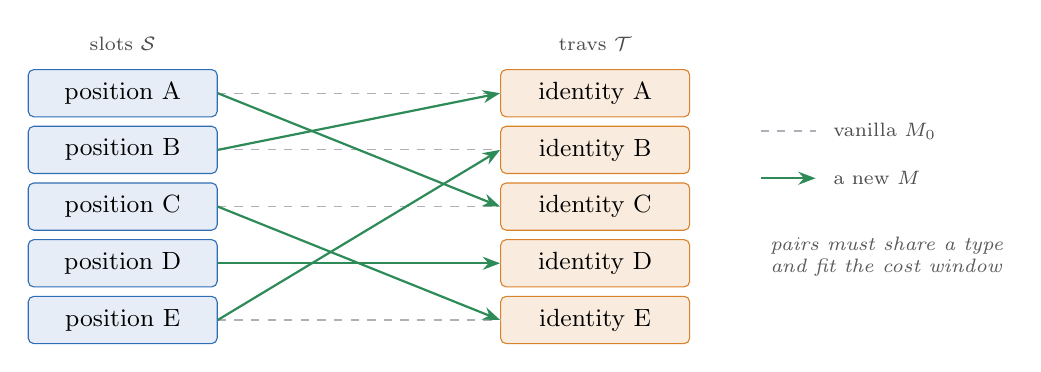
\begin{tikzpicture}[x=1cm,y=1cm]
\foreach \i/\n in {1/A,2/B,3/C,4/D,5/E} {
  \node[slotn, minimum width=2.4cm] (s\i) at (0,-0.72*\i) {position \n};
  \node[travn, minimum width=2.4cm] (t\i) at (6,-0.72*\i) {identity \n};
}
\foreach \i in {1,...,5} \draw[cgrey!70, dashed] (s\i.east) -- (t\i.west);
\draw[pre, cnew] (s1.east) -- (t3.west);
\draw[pre, cnew] (s2.east) -- (t1.west);
\draw[pre, cnew] (s3.east) -- (t5.west);
\draw[pre, cnew] (s4.east) -- (t4.west);
\draw[pre, cnew] (s5.east) -- (t2.west);
\node[lbl, anchor=south] at (0,-0.3) {slots $\Slots$};
\node[lbl, anchor=south] at (6,-0.3) {travs $\Travs$};
\draw[cgrey!70, dashed] (8.1,-1.2) -- (8.8,-1.2); \node[lbl, anchor=west] at (8.9,-1.2) {vanilla $M_0$};
\draw[pre, cnew] (8.1,-1.8) -- (8.8,-1.8); \node[lbl, anchor=west] at (8.9,-1.8) {a new $M$};
\node[note, anchor=west] at (8.1,-2.8) {pairs must share a type\\and fit the cost window};
\end{tikzpicture}
\caption{The assignment as a bipartite perfect matching. An identity may also stay where it is (D here).}
\label{fig:bipartite}
\end{figure}

\subsection{What a valid assignment must keep}
\label{sec:hard}

\paragraph{Pebbles and contexts.} A \emph{complex sort} (\file{lib/graph/context-sort.lua}, with \code{complex_contexts} and \code{home_contexts}) reaches nodes in \emph{contexts}. A context is a room together with an ability string for isolatability and automatability, written like \texttt{planet:\,vulcanus\,|\,11}. A \emph{pebble} $\peb{v}{c}$ is a node $v$ reached in context $c$, and its \emph{rank} $\rk\peb{v}{c}$ is its position in the sort. ``Earlier'' always means lower rank.

\paragraph{Hard pebbles.} What must survive first pass is decided in one place, \file{randomizations/graph/unified/skeleton/protection.lua}:
\begin{enumerate}
  \item \textbf{Mechanic pebbles.} Their room and automatability are always kept. Isolatability is kept for nodes that declare \code{keep_isolatability = true}, or for every node with \code{constants.keep_isolatability}. An unprotected isolatable pebble only needs its non-isolatable counterpart (\code{is_hard_mechanic_pebble}, \code{kept_part}).
  \item \textbf{Planet-locked recipes} keep every context they have on their planet (\code{planet_locked_recipe_contexts}).
  \item \textbf{Every recipe} that was reachable stays reachable, in at least one context.
\end{enumerate}
Home contexts are never kept for their own sake; they only back the discovery rule. In the measured seeds, the sort had about 275{,}000 pebbles. Of those, 3{,}527--3{,}548 had to be kept exactly and 619--621 recipes had to stay reachable.

\medskip
This definition of ``valid'' is itself newer than the greedy fill, which never had it: \file{protection.lua} landed in the same commit as monotone matching (014b8be). Section~\ref{sec:greedy} shows the greedy's own, weaker notion.

\section{The old approach: a greedy forward fill}
\label{sec:greedy}

This was first pass from August (\texttt{bd888e5}, ``Work on mechanics-aware reservation system'', 7 August) until 26 September. That day \texttt{014b8be} put monotone matching into the experimental copy, and \texttt{b717eda} deleted the greedy paths 17 minutes later. Its last version is \verb|git show b717eda^:randomizations/graph/unified/first-pass-new.lua| (1{,}862 lines). In item-randomizer terms it was a \emph{forward fill}: simulate a playthrough, and at each step put something into a location that's already reachable.

\subsection{How it worked}

\paragraph{Setup.}
\begin{enumerate}
  \item Take a random sort of the vanilla graph, with plain room contexts (no abilities), and order the slots by their first rank.
  \item \emph{Targets:} take the witness (\code{top.path}) of the starting planet's science packs. The mechanic nodes on it (plus nodes flagged \code{important}), in sort order, form a list, and the first one not yet reached is the \emph{current mechanic}.
  \item For each identity, record the mechanics it reaches first: a breadth-first search to depth 20 that doesn't pass through mechanics.
  \item Build the split graph (Figure~\ref{fig:split}) with every slot/trav connection cut, and sort it.
\end{enumerate}

\paragraph{Its notion of ``reachable''.} A slot counted as reachable if it's an OR node with a head prerequisite or any prerequisite with \emph{some} context, or an AND node whose prerequisites share \emph{some} context (\code{slot_absolute_reachable}). An identity counted as reachable if it's an OR node (always), or an AND node whose fixed prerequisites share some context (\code{trav_absolute_reachable}). Both are yes/no questions about whether there's any context at all.

\paragraph{Main loop} (once per slot, Figure~\ref{fig:greedy}).
\begin{enumerate}
  \item Take the earliest unassigned, reachable slot.
  \item Walk the free, reachable identities in one fixed shuffled order and take the first \emph{compatible} one (\code{is_compatible}). It must be the same type, have the same first-reached mechanics (for non-items), and fit the cost window (for items). For ore slots, a useless identity was rejected 90\% of the time.
  \item If the identity helps the current mechanic, \emph{connect} it: add base $\to$ head and update the sort incrementally. The current mechanic moves on as soon as it has any context. Otherwise, \emph{reserve} it: record the pair but don't connect it, so it adds nothing to the world yet.
  \item If no pair fits, run the \emph{reservation loop}:
  \begin{enumerate}[label=(\alph*)]
    \item connect a reserved pair whose identity helps the current mechanic;
    \item else swap a free helping identity into a reserved slot;
    \item else build a chain of swaps through reserved slots;
    \item else connect the oldest reservation anyway.
  \end{enumerate}
  Then try again, up to 10{,}000 times per slot.
  \item If it's still stuck: below 50\% of slots assigned, the attempt fails and unified retries. Above 50\%, it turns the reachability checks off (``desperation'') and continues. If it gets stuck again, it fails.
\end{enumerate}

\paragraph{End.} Connect the remaining reservations, sort again, and return. The committed version had no check of what the result kept. The experimental copy added one (\code{GATE_MECHANIC_CONTEXTS}) together with complex contexts, and that check is what exposed the losses below.

\begin{figure}[tbp]
\centering
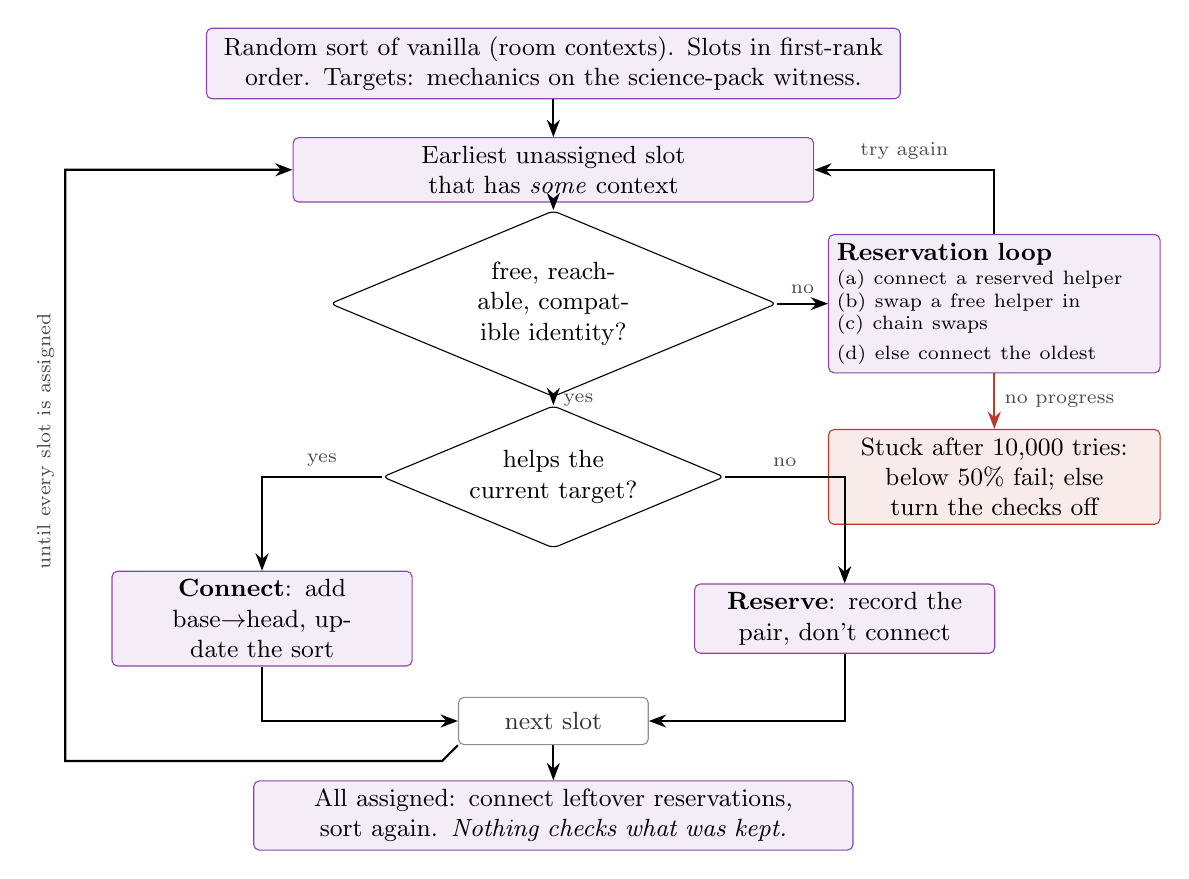
\begin{tikzpicture}[x=1cm,y=1cm, every node/.append style={font=\small}]
\node[oldn, text width=8.6cm] (setup) at (0,0) {Random sort of vanilla (room contexts). Slots in first-rank order. Targets: mechanics on the science-pack witness.};
\node[oldn, text width=6.4cm] (pick) at (0,-1.35) {Earliest unassigned slot that has \emph{some} context};
\node[dec, text width=2.9cm] (d1) at (0,-3.05) {free, reachable, compatible identity?};
\node[dec, text width=2.5cm] (d2) at (0,-5.25) {helps the current target?};
\node[oldn, text width=3.6cm] (connect) at (-3.7,-7.05) {\textbf{Connect}: add base$\to$head, update the sort};
\node[oldn, text width=3.6cm] (reserve) at (3.7,-7.05) {\textbf{Reserve}: record the pair, don't connect};
\node[plain, text width=2.2cm] (next) at (0,-8.35) {next slot};
\node[oldn, text width=7.4cm] (end) at (0,-9.55) {All assigned: connect leftover reservations, sort again. \emph{Nothing checks what was kept.}};
\node[oldn, text width=4.0cm, align=left] (loop) at (5.6,-3.05) {\textbf{Reservation loop}\\[1pt]\scriptsize (a) connect a reserved helper\\ (b) swap a free helper in\\ (c) chain swaps\\ (d) else connect the oldest};
\node[badn, text width=4.0cm] (stuck) at (5.6,-5.25) {Stuck after 10{,}000 tries: below 50\% fail; else turn the checks off};
\draw[pre] (setup) -- (pick);
\draw[pre] (pick) -- (d1);
\draw[pre] (d1) -- node[right, lbl, pos=0.35] {yes} (d2);
\draw[pre] (d1) -- node[above, lbl] {no} (loop);
\draw[pre] (loop.north) |- node[above, lbl, pos=0.75] {try again} (pick.east);
\draw[pre, draw=cbad] (loop) -- node[right, lbl] {no progress} (stuck);
\draw[pre] (d2.west) -| node[above, lbl, pos=0.25] {yes} (connect.north);
\draw[pre] (d2.east) -| node[above, lbl, pos=0.25] {no} (reserve.north);
\draw[pre] (connect.south) |- (next.west);
\draw[pre] (reserve.south) |- (next.east);
\draw[pre] (next) -- (end);
\draw[pre] (next.south west) -- ++(-0.2,-0.2) -| (-6.2,-1.35) -- (pick.west);
\node[lbl, rotate=90] at (-6.45,-4.8) {until every slot is assigned};
\end{tikzpicture}
\caption{The greedy forward fill's control flow (\texttt{b717eda\^{}}). Reservations steered progress toward the next targeted mechanic, and the reservation loop was the only way out of a dead end.}
\label{fig:greedy}
\end{figure}

\subsection{Why it lost contexts}
\label{sec:greedy-losses}

\begin{enumerate}[leftmargin=*]
  \item \textbf{Yes/no reachability.} A slot that has \emph{some} context passes, even if it never has the context the identity is needed in. There are two ways this goes wrong (Figure~\ref{fig:greedy-loss}). In a \emph{static mismatch}, the slot is never reached in that context at all. In a \emph{context-local cycle}, the slot is reached in that context only through the identity it's about to hold.
  \item \textbf{Targets by node, only on the science path.} A mechanic counted as done once it had \emph{any} context, so a later mechanic that needed it in another room was never protected. Mechanics off the starting planet's science-pack witness weren't targeted at all. The experimental copy's comment on \code{TARGET_ALL_MECHANICS} says ``untargeted ones weren't protected at all''.
  \item \textbf{No fallback.} A partial assignment that can't be extended is a dead end. The reservation loop only reshuffles pairs that are already placed; it never goes back to a known good state. Desperation mode fills the rest without checks.
  \item \textbf{Reproducibility.} The ore roll used \code{math.random} rather than the mod's seeded \code{rng}, and rolled again every time the same pair was checked. The experimental copy's fix comment records this.
\end{enumerate}

\begin{factbox}
\textbf{Measured on 25 September} (experimental copy with complex contexts and a gate; from that investigation's notes, not re-measured here):
\begin{itemize}
  \item 7--12 misplaced identities per seed explained \emph{all} of the roughly 466 lost mechanic pebbles, and every lost pebble was an isolatable context. The roots were static mismatches or context-local cycles. The notes' example is coal's identity landing in the roboport's position, which broke a Vulcanus context.
  \item Adding a filter so the greedy only used slots reachable in the needed isolatable rooms made it stall at 77--81\% on all 10 retries.
\end{itemize}
So the greedy couldn't be patched to keep isolatability. Either it lost contexts or it got stuck.
\end{factbox}

\begin{figure}[tbp]
\centering
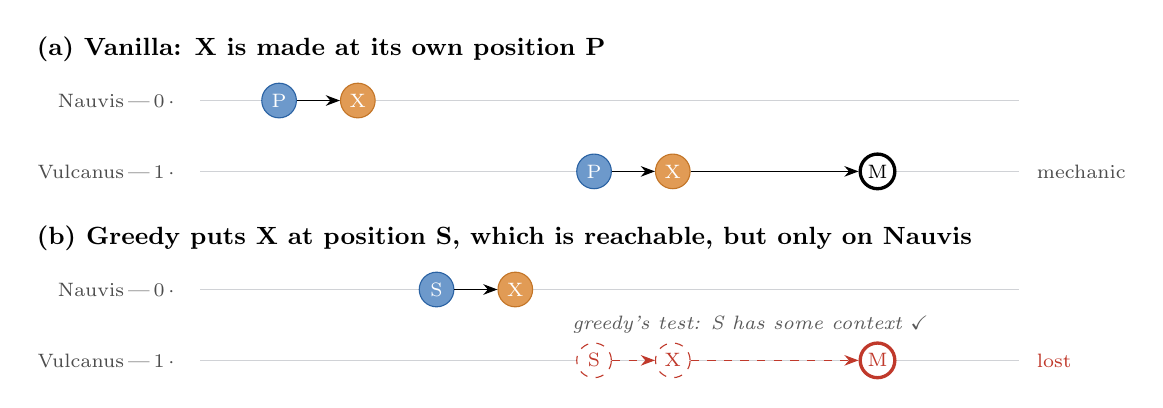
\begin{tikzpicture}[x=1cm,y=1cm]
\def\lanes#1{%
  \node[lbl, anchor=east] at (-0.2,0) {Nauvis\,|\,0\,$\cdot$};
  \node[lbl, anchor=east] at (-0.2,-0.9) {Vulcanus\,|\,1\,$\cdot$};
  \draw[cgrey!40] (0,0) -- (10.4,0);
  \draw[cgrey!40] (0,-0.9) -- (10.4,-0.9);
  \node[anchor=west, font=\small\bfseries] at (-2.2,0.65) {#1};
}
% (a) vanilla
\lanes{(a) Vanilla: X is made at its own position P}
\node[spebble] (p1) at (1.0,0) {P};
\node[tpebble] (x1) at (2.0,0) {X};
\node[spebble] (p2) at (5.0,-0.9) {P};
\node[tpebble] (x2) at (6.0,-0.9) {X};
\node[pebble, very thick] (m1) at (8.6,-0.9) {M};
\draw[thinpre] (p1) -- (x1);
\draw[thinpre] (p2) -- (x2);
\draw[thinpre] (x2) -- (m1);
\node[lbl, anchor=west] at (10.5,-0.9) {mechanic};
% (b) after greedy
\begin{scope}[yshift=-2.4cm]
\lanes{(b) Greedy puts X at position S, which is reachable, but only on Nauvis}
\node[spebble] (s1) at (3.0,0) {S};
\node[tpebble] (x3) at (4.0,0) {X};
\node[ghost, draw=cbad, text=cbad] (s2) at (5.0,-0.9) {S};
\node[ghost, draw=cbad, text=cbad] (x4) at (6.0,-0.9) {X};
\node[pebble, very thick, draw=cbad, text=cbad] (m2) at (8.6,-0.9) {M};
\draw[thinpre] (s1) -- (x3);
\draw[thinpre, draw=cbad, dashed] (s2) -- (x4);
\draw[thinpre, draw=cbad, dashed] (x4) -- (m2);
\node[lbl, anchor=west, text=cbad] at (10.5,-0.9) {lost};
\node[note, anchor=west] at (4.6,-0.45) {greedy's test: S has some context \checkmark};
\end{scope}
\end{tikzpicture}
\caption{How yes/no reachability loses a context. The lanes are contexts (room\,|\,isolatability\,automatability) and rank grows to the right. In (b), S has no Vulcanus-isolatable pebble, so X doesn't either, and neither does the mechanic M that needed it. In a context-local cycle, S \emph{would} reach Vulcanus, but only by using X there, so moving X to S breaks the loop.}
\label{fig:greedy-loss}
\end{figure}

\section{The new approach: monotone matching}
\label{sec:matching}

\noindent\textbf{Code:} \file{randomizations/graph/unified/first-pass-new.lua} does the setup, the split and the final gate. \file{randomizations/graph/unified/skeleton/monotone-matching.lua} runs the rounds. \textbf{History:} it landed in \texttt{014b8be} (26 Sep, 00:31) and became the only first pass in \texttt{b717eda} (00:48). Mechanics-aware needs and the reflection model came in \texttt{85efe29}, home contexts in \texttt{8f5e55d}, and starting ores and coal's fuel in \texttt{86362b2}.

\subsection{The idea: move between valid matchings}

The greedy fill searched through \emph{partial} assignments, and most of them can't be completed in a way that keeps everything. Monotone matching searches through \emph{complete, valid} assignments only. It starts from the one assignment known to be valid, vanilla, and makes big random moves. Each move is checked exactly, and a move that fails is simply not taken (Figure~\ref{fig:space}).

\begin{figure}[tbp]
\centering
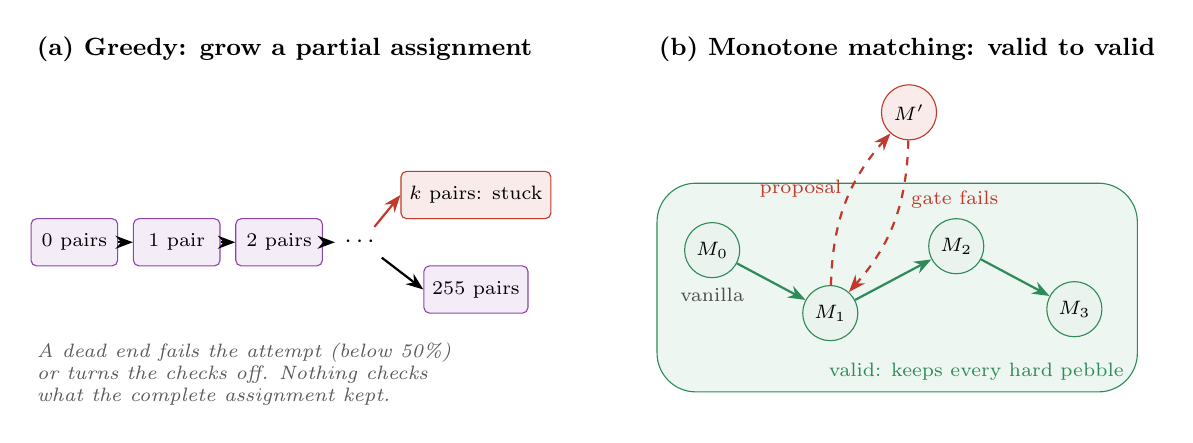
\begin{tikzpicture}[x=1cm,y=1cm]
% ---------------- greedy
\node[anchor=west, font=\small\bfseries] at (-0.3,2.85) {(a) Greedy: grow a partial assignment};
\foreach \i/\t/\x in {0/{0 pairs}/0.3, 1/{1 pair}/1.6, 2/{2 pairs}/2.9} {
  \node[oldn, minimum width=1.1cm] (g\i) at (\x,0.4) {\scriptsize \t};
}
\node[font=\small] (gdots) at (3.95,0.4) {$\cdots$};
\node[badn, minimum width=1.2cm] (gk) at (5.4,1.0) {\scriptsize $k$ pairs: stuck};
\node[oldn, minimum width=1.2cm] (gn) at (5.4,-0.2) {\scriptsize 255 pairs};
\draw[pre] (g0) -- (g1); \draw[pre] (g1) -- (g2); \draw[pre] (g2) -- (gdots);
\draw[pre, draw=cbad] (gdots) -- (gk.west);
\draw[pre] (gdots) -- (gn.west);
\node[note, anchor=north west] at (-0.3,-0.75) {A dead end fails the attempt (below 50\%)\\or turns the checks off. Nothing checks\\what the complete assignment kept.};
% ---------------- matching
\begin{scope}[xshift=7.9cm]
\node[anchor=west, font=\small\bfseries] at (-0.3,2.85) {(b) Monotone matching: valid to valid};
\draw[rounded corners=14pt, fill=cnew!8, draw=cnew] (-0.2,-1.5) rectangle (5.9,1.15);
\node[lbl, text=cnew, anchor=south east] at (5.85,-1.48) {valid: keeps every hard pebble};
\node[newn, circle, inner sep=1pt, minimum size=7mm] (m0) at (0.5,0.3) {\scriptsize $M_0$};
\node[newn, circle, inner sep=1pt, minimum size=7mm] (m1) at (2.0,-0.5) {\scriptsize $M_1$};
\node[newn, circle, inner sep=1pt, minimum size=7mm] (m2) at (3.6,0.35) {\scriptsize $M_2$};
\node[newn, circle, inner sep=1pt, minimum size=7mm] (m3) at (5.1,-0.45) {\scriptsize $M_3$};
\node[badn, circle, inner sep=1pt, minimum size=7mm] (mx) at (3.0,2.05) {\scriptsize $M'$};
\draw[pre, draw=cnew] (m0) -- (m1);
\draw[pre, draw=cnew] (m1) -- (m2);
\draw[pre, draw=cnew] (m2) -- (m3);
\draw[pre, draw=cbad, dashed] (m1) to[bend left=20] node[left, lbl, text=cbad, pos=0.6] {proposal} (mx);
\draw[pre, draw=cbad, dashed] (mx) to[bend left=20] node[right, lbl, text=cbad, pos=0.35] {gate fails} (m1);
\node[lbl, anchor=north] at (m0.south) {vanilla};
\end{scope}
\end{tikzpicture}
\caption{The two search spaces. In (b), every round ends at a valid matching: either the proposal passed the gate, or the round keeps the matching it started with. Failed proposals are rare: 4 of the 74 logged rounds (Section~\ref{sec:measure}).}
\label{fig:space}
\end{figure}

\begin{proposition}[Every round ends valid]
\label{prop:invariant}
Let $\Hard$ be the hard pebbles of the vanilla matching $M_0$ (Section~\ref{sec:hard}), computed once before round 1. Assume the set of pebbles a complex sort reaches doesn't depend on the sort's random order. Then every round of \code{matching.run} returns a matching that keeps all of $\Hard$: each exact pebble in its context, and each recipe in at least one context.
\end{proposition}
\begin{proof}
By induction on rounds. $M_0$ keeps $\Hard$, because $\Hard$ is read off $M_0$'s own sort. Round $r$ returns one of two things. The first is a proposal whose fresh sort lost nothing in $\Hard$: that's exactly the gate's condition, and by the assumption, one sort speaks for all of them. The second, when refinement gives up, is the matching $M_{r-1}$ the round started with.
\end{proof}

\noindent The assumption is what home contexts were introduced for. The old tech discovery rule depended on order, so two sorts of one graph could disagree. First pass also runs a second gate after the rounds, against the original graph (Section~\ref{sec:after}). So even if the assumption failed somewhere, a bad result would make the attempt retry rather than ship. Note what the proposition does \emph{not} say: it doesn't say a proposal is likely to pass. That's the job of the proofs and the rank rule, and it's measured rather than proved (Section~\ref{sec:measure}).

\subsection{One round}

\begin{figure}[tbp]
\centering
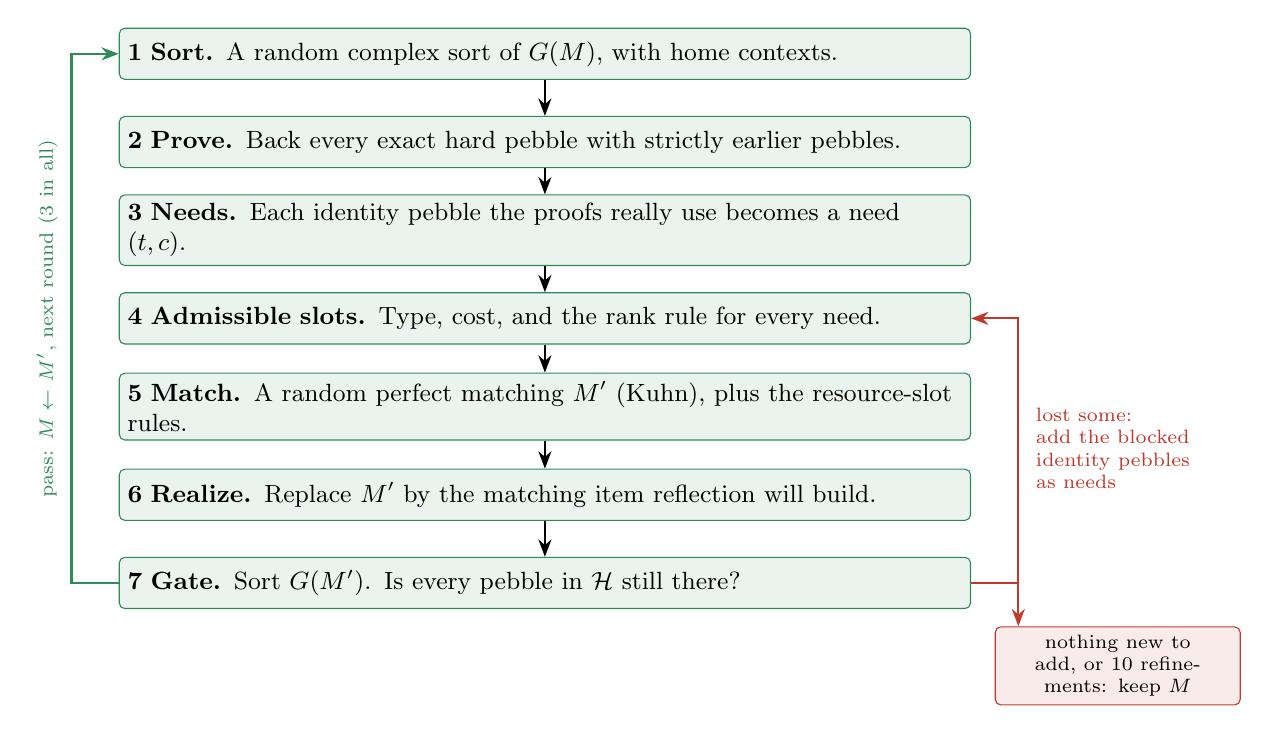
\begin{tikzpicture}[x=1cm,y=1cm, every node/.append style={font=\small}]
\tikzset{rstep/.style={newn, text width=10.6cm, align=left, minimum height=6.5mm}}
\node[rstep] (s1) at (0,0)      {\textbf{1\;Sort.} A random complex sort of $G(M)$, with home contexts.};
\node[rstep] (s2) at (0,-1.12)   {\textbf{2\;Prove.} Back every exact hard pebble with strictly earlier pebbles.};
\node[rstep] (s3) at (0,-2.24)   {\textbf{3\;Needs.} Each identity pebble the proofs really use becomes a need $(t,c)$.};
\node[rstep] (s4) at (0,-3.36)   {\textbf{4\;Admissible slots.} Type, cost, and the rank rule for every need.};
\node[rstep] (s5) at (0,-4.48)   {\textbf{5\;Match.} A random perfect matching $M'$ (Kuhn), plus the resource-slot rules.};
\node[rstep] (s6) at (0,-5.60)   {\textbf{6\;Realize.} Replace $M'$ by the matching item reflection will build.};
\node[rstep] (s7) at (0,-6.72)   {\textbf{7\;Gate.} Sort $G(M')$. Is every pebble in $\Hard$ still there?};
\foreach \a/\b in {s1/s2,s2/s3,s3/s4,s4/s5,s5/s6,s6/s7} \draw[pre] (\a) -- (\b);
\draw[pre, draw=cnew] (s7.west) -- ++(-0.6,0) |- (s1.west);
\node[lbl, text=cnew, rotate=90, anchor=south] at ($(s1.west)+(-0.65,-3.36)$) {pass: $M \gets M'$, next round (3 in all)};
\draw[pre, draw=cbad] (s7.east) -- ++(0.6,0) |- (s4.east);
\node[lbl, text=cbad, anchor=west, align=left] at ($(s4.east)+(0.7,-1.65)$) {lost some:\\add the blocked\\identity pebbles\\as needs};
\node[badn, text width=2.9cm, font=\scriptsize, anchor=north west] (keep) at ($(s7.east)+(0.3,-0.55)$) {nothing new to add, or 10 refinements: keep $M$};
\draw[pre, draw=cbad] ($(s7.east)+(0.6,0)$) -- ($(s7.east)+(0.6,-0.55)$);
\end{tikzpicture}
\caption{One round of \code{matching.run}. Steps 1--3 run once per round. Steps 4--7 repeat for each refinement. In 70 of 74 logged rounds, the first proposal passed. In the other 4, refinement found nothing to add, and the round kept $M$.}
\label{fig:round}
\end{figure}

\subsubsection{Steps 1--2: sort, then prove the hard pebbles}

Each round takes a fresh random complex sort of the current graph $G(M)$. It then proves the \emph{exact} hard pebbles in it: protected mechanic pebbles and planet-locked recipe pebbles. Recipes are left to the gate, since needs for them would be too strict. The prover (\code{make_prover}) builds a \emph{backing} for each goal out of strictly earlier pebbles, like promotion's \code{compute_support}:
\begin{itemize}
  \item \textbf{AND node:} every prerequisite needs an earlier pebble that is itself established.
  \item \textbf{OR node:} the providers' earlier pebbles are tried in rank order, earliest first. If one can't be established, the next one is tried. This backtracking is what \code{top.path}'s single earliest-provider witness lacks.
  \item \textbf{Nodes that change contexts} (forgetters and emitters): try the incoming contexts that turn into this one, earliest first.
  \item \textbf{Technologies} can also be backed through the discovery rule (\code{top.discovery_candidates}): an earlier pebble of the tech itself in a home context, plus an earlier pebble of a discoverer of the room.
\end{itemize}
Results are memoized. A pebble that's still being evaluated counts as unproven, so backings can't loop. The result is the \emph{closure}: every pebble the proofs use. In the measured runs, every exact hard pebble was proven in every round, and the closure held about 26{,}000--28{,}500 pebbles.

\subsubsection{Step 3: needs}

A \emph{need} is a pair $(t,c)$: identity $t$ must still be available in context $c$. Needs come only from identity (trav) pebbles in the closure, and only from real uses (\code{needs_from_proof}, Figure~\ref{fig:needs}):
\begin{itemize}
  \item A trav pebble counts if some user in the proof leads to a real use of the identity. Users on the trav's own launch chain, or the trav itself, are followed further.
  \item \emph{Delivered} contexts aren't needs. They're backed through the trav's own launch chain (trav $\to$ item-launch $\to$ item-deliver $\to$ trav), so they follow from the context the item was launched from.
  \item Sometimes a trav's only use in another room is feeding its own slot's consumers there, by delivery. Then the requirement moves to the \emph{slot}: whatever identity it holds must be launchable (\code{requires_launchable}), and the identity itself isn't pinned.
\end{itemize}
Because the prover picks one provider per OR, an identity is pinned only where the proof actually uses it. If another provider comes first in the next round's sort, the old one is free again. With these rules, 90--100 of the 255 identities had needs in each measured round, with 215--228 needs between them. The other 155--165 identities were free to go anywhere their type and cost allowed.

\begin{figure}[tbp]
\centering
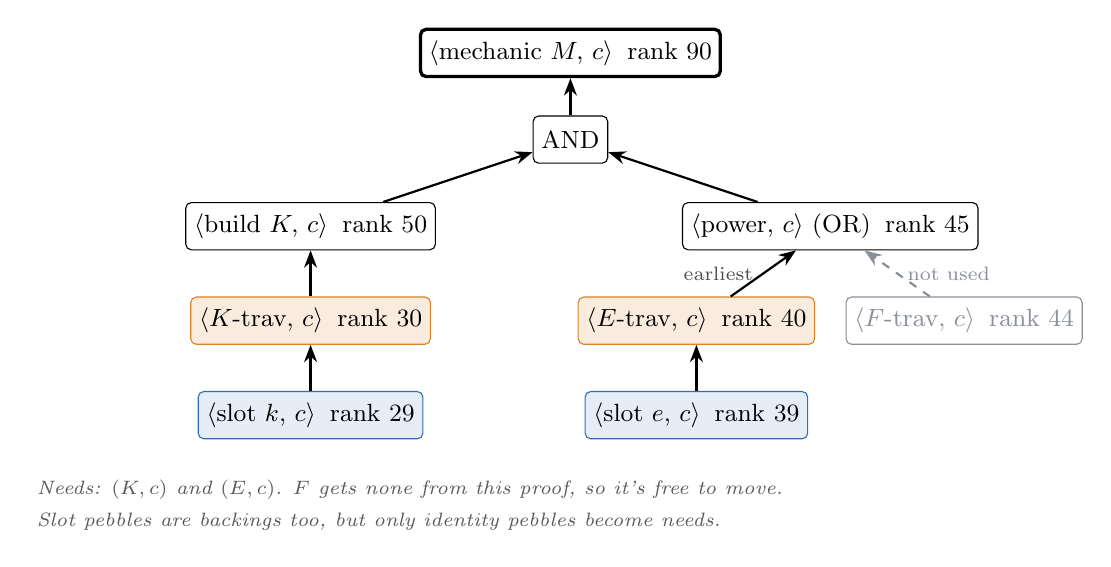
\begin{tikzpicture}[x=1cm,y=1cm, every node/.append style={font=\small}]
\node[box, very thick] (g) at (0,0) {$\peb{\text{mechanic }M}{c}$\;\;rank 90};
\node[box] (and) at (0,-1.1) {AND};
\node[box] (bk) at (-3.3,-2.2) {$\peb{\text{build }K}{c}$\;\;rank 50};
\node[box] (pw) at (3.3,-2.2) {$\peb{\text{power}}{c}$ (OR)\;\;rank 45};
\node[travn] (tk) at (-3.3,-3.4) {$\peb{K\text{-trav}}{c}$\;\;rank 30};
\node[travn] (te) at (1.6,-3.4) {$\peb{E\text{-trav}}{c}$\;\;rank 40};
\node[travn, draw=cgrey, fill=white, text=cgrey] (tf) at (5.0,-3.4) {$\peb{F\text{-trav}}{c}$\;\;rank 44};
\node[slotn] (sk) at (-3.3,-4.6) {$\peb{\text{slot }k}{c}$\;\;rank 29};
\node[slotn] (se) at (1.6,-4.6) {$\peb{\text{slot }e}{c}$\;\;rank 39};
\draw[pre] (and) -- (g);
\draw[pre] (bk) -- (and);
\draw[pre] (pw) -- (and);
\draw[pre] (tk) -- (bk);
\draw[pre] (te) -- node[left, lbl] {earliest} (pw);
\draw[pre, draw=cgrey, dashed] (tf) -- node[right, lbl, text=cgrey] {not used} (pw);
\draw[pre] (sk) -- (tk);
\draw[pre] (se) -- (te);
\node[note, anchor=west] at (-6.9,-5.55) {Needs: $(K, c)$ and $(E, c)$. $F$ gets none from this proof, so it's free to move.};
\node[note, anchor=west] at (-6.9,-5.95) {Slot pebbles are backings too, but only identity pebbles become needs.};
\end{tikzpicture}
\caption{Needs come from a proof, not from every route. Power has two providers here. The prover takes the earliest one that it can itself prove ($E$), so only $E$ is pinned in context $c$. The ranks are made up for the example.}
\label{fig:needs}
\end{figure}

\subsubsection{Step 4: admissible slots, and the rank rule}

\begin{definition}[Admissible]
Let $\rk$ be the ranks in this round's sort of $G(M)$. Slot $s$ is \emph{admissible} for trav $t$ if $s$ has the same type as $t$, \code{pair_ok}$(s,t)$ holds, and
\[
  \forall\, (t,c)\in\Need:\qquad \peb{s}{c}\text{ exists and }\ \rk\peb{s}{c} \;<\; \rk\peb{t}{c}.
\]
If a slot requires a launchable identity, $t$ must also be launchable. The trav's current slot $M^{-1}(t)$ is always admissible.
\end{definition}

\noindent In words, a needed identity may move only to a position that, in every context it's needed in, was reached \emph{before} the identity itself was reached through its current position. In the next graph, the identity's supply in context $c$ then comes from a pebble that was earlier than the identity. The proof's backing through $t$ only gets \emph{earlier}, and that's what \emph{monotone} refers to. It's the same ``strictly earlier'' condition that makes promotion's promises well-founded.

\begin{figure}[tbp]
\centering
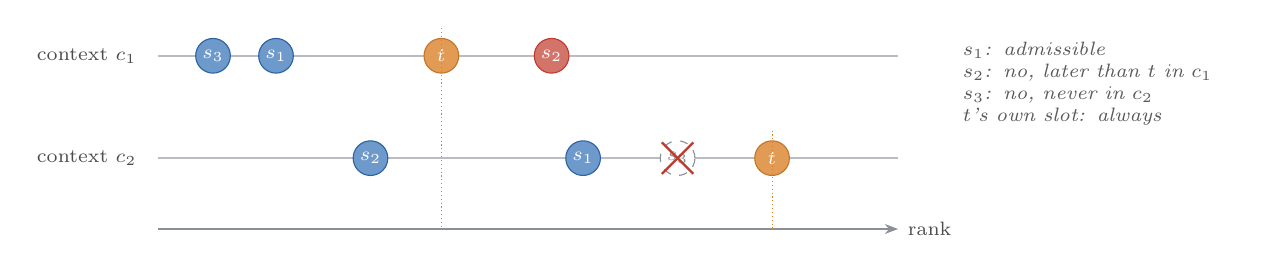
\begin{tikzpicture}[x=1cm,y=1cm]
\foreach \y/\c in {0/c_1, -1.3/c_2} {
  \draw[cgrey!60, thick] (0,\y) -- (9.4,\y);
  \node[lbl, anchor=east] at (-0.15,\y) {context $\c$};
}
\draw[-{Stealth}, cgrey] (0,-2.2) -- (9.4,-2.2) node[lbl, anchor=west] {rank};
\node[tpebble] (x1) at (3.6,0) {$t$};
\node[tpebble] (x2) at (7.8,-1.3) {$t$};
\node[spebble] at (1.5,0) {$s_1$};
\node[spebble] at (5.4,-1.3) {$s_1$};
\node[spebble, fill=cbad!70, draw=cbad] at (5.0,0) {$s_2$};
\node[spebble] at (2.7,-1.3) {$s_2$};
\node[spebble] at (0.7,0) {$s_3$};
\node[ghost] at (6.6,-1.3) {$s_3$};
\draw[cbad, thick] (6.4,-1.5) -- (6.8,-1.1) (6.4,-1.1) -- (6.8,-1.5);
\draw[densely dotted, ctrav] (3.6,0.35) -- (3.6,-2.2);
\draw[densely dotted, ctrav] (7.8,-0.95) -- (7.8,-2.2);
\node[note, anchor=north west, text width=3.4cm] at (10.1,0.3) {$s_1$: admissible\\$s_2$: no, later than $t$ in $c_1$\\$s_3$: no, never in $c_2$\\$t$'s own slot: always};
\end{tikzpicture}
\caption{The rank rule for an identity $t$ with needs in two contexts. A slot must beat $t$ in \emph{every} needed context.}
\label{fig:rankrule}
\end{figure}

\noindent In the measured rounds, identities with needs had on average 38--69 admissible slots besides their own, and free identities about 217. Between 2 and 9 identities per round had none besides their own, so they stayed put that round.

\subsubsection{Step 5: a random perfect matching}

The admissibility graph always has a perfect matching, because the current matching is one (each trav's current slot is admissible). \code{random_matching} finds one with Kuhn's augmenting-path algorithm. It visits the travs in random order and tries each trav's admissible slots in random order, with its current slot \emph{last}, which pushes identities to move. Augmenting paths find a perfect matching whenever one exists, so this step never fails.

\paragraph{Resource slots.} Item reflection doesn't swap two useless items, and ores count as useless, so an ore patch would usually keep mining what it did. The matching steers resource slots toward \emph{new, interesting} identities. An identity is new and interesting for a resource slot if it's not useless (\code{dutils.is_useless_item}) and not the slot's own identity.
\begin{enumerate}
  \item A resource slot that already mines something new keeps its identity, so no round undoes it.
  \item Every other resource slot, in random order, tries up to 5 random admissible new identities. It keeps one only if a perfect matching still exists with it.
  \item After Kuhn's algorithm finishes, a breadth-first search looks for a \emph{cycle of moves} for each resource slot still without a new identity. Each identity on the cycle moves to a slot it's admissible for, and the cycle ends with a new identity moving into the resource slot, without making another resource slot stop mining something new (Figure~\ref{fig:cycle}).
\end{enumerate}

\begin{figure}[tbp]
\centering
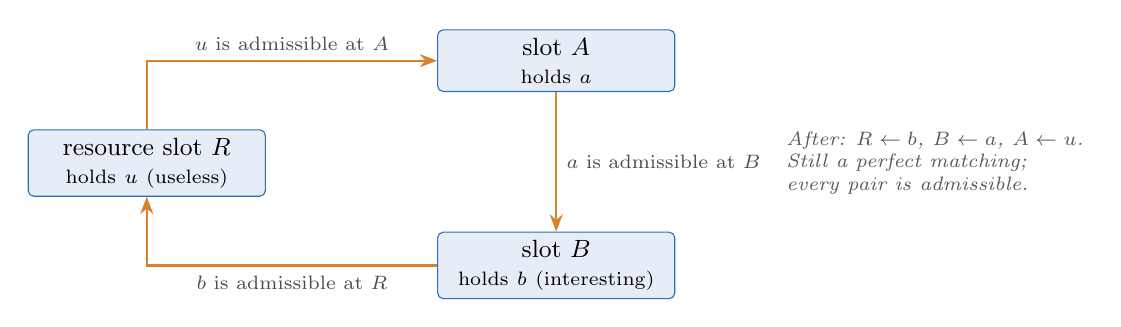
\begin{tikzpicture}[x=1cm,y=1cm]
\node[slotn, text width=2.8cm] (r) at (0,0) {resource slot $R$\\[-1pt]{\scriptsize holds $u$ (useless)}};
\node[slotn, text width=2.8cm] (a) at (5.2,1.3) {slot $A$\\[-1pt]{\scriptsize holds $a$}};
\node[slotn, text width=2.8cm] (b) at (5.2,-1.3) {slot $B$\\[-1pt]{\scriptsize holds $b$ (interesting)}};
\draw[pre, draw=ctrav] (r.north) |- node[above, lbl, pos=0.75] {$u$ is admissible at $A$} (a.west);
\draw[pre, draw=ctrav] (a.south) -- node[right, lbl] {$a$ is admissible at $B$} (b.north);
\draw[pre, draw=ctrav] (b.west) -| node[below, lbl, pos=0.25] {$b$ is admissible at $R$} (r.south);
\node[note, anchor=west] at (8.0,0) {After: $R\gets b$, $B\gets a$, $A\gets u$.\\Still a perfect matching;\\every pair is admissible.};
\end{tikzpicture}
\caption{Cycle repair for a resource slot. The search is breadth-first from $R$ over ``the identity at this slot may move to that slot''.}
\label{fig:cycle}
\end{figure}

\subsubsection{Steps 6--7: realize, gate, refine}
\label{sec:gate}

\paragraph{Realize.} Reflection places useless identities differently from the matching (\code{dutils.realized_item_assignment}), so the proposal is replaced by the matching reflection will actually build. That's still a perfect matching, and realizing $M_0$ gives $M_0$ back. So the gate judges the game that will actually be built, not an idealized one. The same commit (\texttt{85efe29}) fixed a second place where the model and the game disagreed, in the split. Mining drops of player creations and of tiles now belong to the identity. Before that fix, the Fulgoran ruin's stone brick drop was modeled as a position, which lost about 101 isolated-Fulgora contexts whenever that position held something else.

\paragraph{Gate.} Connect $M'$, sort $G(M')$ from scratch, and list the hard pebbles that are missing (\code{lost_pebbles}). An exact pebble is lost if its context is missing, and a recipe is lost only if it has no pebble at all. If nothing is lost, the proposal is accepted.

\paragraph{Refine.} Otherwise, for each lost pebble, the gate takes its witness in the round's \emph{starting} graph (\code{top.path}). The identity pebbles on that witness that the new sort no longer reaches become extra needs (\code{blocked_travs}). Then steps 4--7 run again with a new random stream. Needs only grow, and each trav's current slot stays admissible whatever its needs, so a perfect matching still exists. If refinement can't add a new need, or after 10 refinements, the round keeps $M$.

\paragraph{Why proposals can fail at all.} The rank rule checks the moved identity's needs, but not the new slot's \emph{own} backing. That backing may use other identities, and those may move too (Figure~\ref{fig:gap}). The gate closes that gap exactly. Refinement closes it only when the missing piece shows up on the lost pebble's old witness. In the failure drawn below, the witness runs through $t$'s old slot, not through $y$, so refinement finds nothing new and the round keeps $M$. All four failed proposals in the logs ended exactly like that, with refinement adding no needs (Table~\ref{tab:failed}).

\begin{figure}[tbp]
\centering
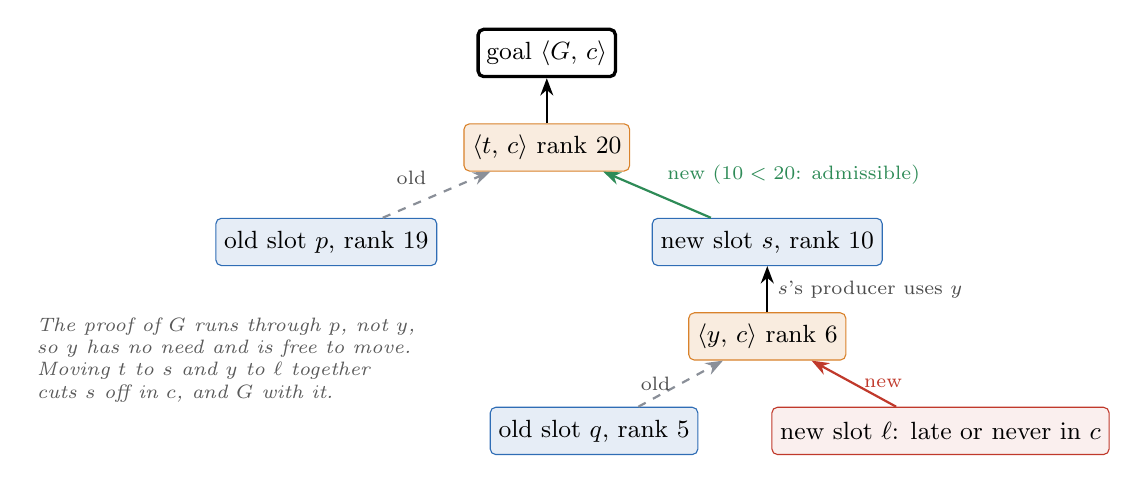
\begin{tikzpicture}[x=1cm,y=1cm, every node/.append style={font=\small}]
\node[box, very thick] (g) at (0,0) {goal $\peb{G}{c}$};
\node[travn] (t) at (0,-1.2) {$\peb{t}{c}$ rank 20};
\node[slotn] (p) at (-2.8,-2.4) {old slot $p$, rank 19};
\node[slotn] (s) at (2.8,-2.4) {new slot $s$, rank 10};
\node[travn] (y) at (2.8,-3.6) {$\peb{y}{c}$ rank 6};
\node[slotn] (q) at (0.6,-4.8) {old slot $q$, rank 5};
\node[slotn, draw=cbad, fill=cbad!8] (l) at (5.0,-4.8) {new slot $\ell$: late or never in $c$};
\draw[pre] (t) -- (g);
\draw[pre, draw=cgrey, dashed] (p) -- node[above left, lbl] {old} (t);
\draw[pre, draw=cnew] (s) -- node[above right, lbl, text=cnew] {new ($10<20$: admissible)} (t);
\draw[pre] (y) -- node[right, lbl] {$s$'s producer uses $y$} (s);
\draw[pre, draw=cgrey, dashed] (q) -- node[left, lbl] {old} (y);
\draw[pre, draw=cbad] (l) -- node[right, lbl, text=cbad] {new} (y);
\node[note, anchor=west] at (-6.6,-3.9) {The proof of $G$ runs through $p$, not $y$,\\so $y$ has no need and is free to move.\\Moving $t$ to $s$ and $y$ to $\ell$ together\\cuts $s$ off in $c$, and $G$ with it.};
\end{tikzpicture}
\caption{The gap the gate closes. Each move looks fine by itself, but together they break a slot's own backing.}
\label{fig:gap}
\end{figure}

\subsection{After the rounds}
\label{sec:after}

\code{first_pass.execute} connects the final matching and sorts the split graph once more. It then runs its own gate against the \emph{original} graph's sort: every mechanic pebble keeps its protected part (\code{protection.kept_part}), and every planet-locked recipe keeps its contexts. If anything is lost, it returns \code{false} and unified randomization retries the attempt. Otherwise it returns the matching (\code{slot_to_trav}, \code{trav_to_slot}), the split graph, and its sort, which promotion reasons over. It also returns the planet-locked contexts and the ``mechanics sets'' that item reflection uses to scale costs. That last piece is a leftover from the greedy: the depth-20 breadth-first search now only feeds cost scaling.

\begin{factbox}
\textbf{Work in progress when this was written} (uncommitted, in another session):
\begin{itemize}
  \item \emph{Entity positions.} Entity randomization flags \code{entity-build-item} nodes as \code{first_pass_entity}, so first pass also decides which entity is built where an item used to place another one. Mine-back heads are \emph{coupled} to their slot (\code{connect_extra}). Their cost rule uses the own item's cost within \code{constants.entity_cost_tolerance}.
  \item \emph{Debt goals.} With planetary changes superposed (\code{SUPERPOSED}, off by default), goals that only the older world reaches must stay reachable with its debt. They're gated on a superposed sort and refined from its witnesses. This is step 2 of the plan in the context-shift report.
\end{itemize}
Neither changes the algorithm above. They add slots and goals to it.
\end{factbox}

\section{Side by side: is it a completely new approach?}
\label{sec:compare}

\subsection{What was kept, changed, removed and added}

Table~\ref{tab:lineage} sorts every part of first pass into four groups: kept, changed, removed and new. It compares the last greedy version (\texttt{b717eda\^{}}) with the current working tree.

\begin{table}[H]
\centering\small
\begin{tabularx}{\textwidth}{@{}p{2.1cm}L@{}}
\toprule
\textbf{Kept} & The slot/trav split and its edge rules (Figure~\ref{fig:split}). Which nodes take part. The first random sort of vanilla, and its science-tier variant for Pyanodon's. The cost window, which moved from \code{is_compatible}'s item branch into \code{cost_ok}. The depth-20 ``mechanics reached first'' search, which now only feeds item reflection's cost scaling. The return values, so promotion and the handlers didn't change.\\
\addlinespace
\textbf{Changed} & Sorts now use room \emph{and} ability contexts, plus home contexts. Ore slots used a 90\% reject roll; now they keep new identities, get prefilled, and get cycle repair. The mining exception used to match \code{place_result}; now it's \code{dutils.mining_keeps_item_names}, shared with reflection. Coal used to be a commented-out special case; now its fuel stays on the slot, and \code{pair_ok} applies. Items get the trav $\to$ slot edge, first added in the experimental copy.\\
\addlinespace
\textbf{Removed} & The reachability tests. Reservations and the target-mechanic list from the science-pack witness. The reservation loop and its swap chains. Desperation mode and \code{FAILURE_ACCEPTANCE}. Incremental sort updates while filling. \code{is_compatible}'s same-mechanics and recipe checks. The recipe-first-pass branches (\code{SPECIAL_RECIPE_FIRST_PASS}). The debug walkers. \texttt{b717eda} removed 1{,}530 lines from \file{first-pass-new.lua} and added 121, and it deleted the 2{,}110-line experimental copy.\\
\addlinespace
\textbf{New} & Hard pebbles from \file{protection.lua}, including planet-locked recipes. The backtracking prover and the needs taken from its proofs. The rank rule. The random perfect matching, with resource rules. Realizing the matching the way reflection will. The gate and refinement. Rounds that start from the last valid matching. First pass's own final gate and retry.\\
\bottomrule
\end{tabularx}
\caption{Code lineage from the greedy fill to monotone matching.}
\label{tab:lineage}
\end{table}

\subsection{The answer}

\textbf{Yes, as a search algorithm. No, as a model of the problem.} The \emph{frame} is unchanged: what gets assigned, how the assignment is represented in the graph, and who consumes it. So downstream code (promotion, the handlers, item reflection) didn't have to change when the algorithm was swapped. The \emph{method} was replaced wholesale, not refactored, and no line of the greedy's search loop survives.

It's a different \emph{kind} of algorithm, too:

\begin{itemize}
  \item The greedy was a \textbf{simulation}. It played the game forward and placed things where the player could already reach. That's the classic forward fill used by many item randomizers. Its correctness depended on the simulation's notion of ``reachable'', and that notion was coarser than what the randomizer has to keep.
  \item Monotone matching is a \textbf{certification}. It holds a world known to be completable (the current matching), a sort of it, and a fallback that's always available (the same matching). It only accepts a change backed by strictly earlier pebbles, and then checked exactly.
\end{itemize}

\noindent That second description is also a description of \emph{promotion} (\file{skeleton/promotion.lua}). Promotion's fallback is a recipe's vanilla ingredients. Monotone matching's fallback is the matching it started the round with. Both reason in the same currency: pebbles, ranks, backings, and the protection rules. The context-shift report calls such a triple of world, sort and fallback a \emph{reference}. In those terms, first pass used to be the one part of unified randomization that didn't have one, and now it does.

\begin{table}[H]
\centering\small
\begin{tabularx}{\textwidth}{@{}p{2.8cm}LL@{}}
\toprule
& \textbf{Promotion} (recipes, generic handlers) & \textbf{Monotone matching} (first pass)\\
\midrule
Reference world & first pass's split graph, with its matching & the current matching $M$\\
Sort & one random complex sort & a fresh random complex sort per round\\
What must hold & promised pebbles are well-founded & hard pebbles of $M_0$ are kept\\
A change is proposed when & a candidate's backing is strictly earlier & a needed identity's new slot is strictly earlier\\
Fallback & the recipe's vanilla ingredients & keep $M$\\
Exact check & UNIFIEDCHECK (built game) & the gate (per proposal), then first pass's gate\\
\bottomrule
\end{tabularx}
\caption{Monotone matching reuses promotion's ideas. Both are ``reference'' constructions in the sense of the context-shift report.}
\label{tab:kinship}
\end{table}

\section{Measurements}
\label{sec:measure}

\paragraph{Setup.} These runs used the working tree of 26 September 2026 (HEAD \texttt{fe064cb} plus uncommitted work), Space Age, and the user's startup settings, on seeds 1--3. Measurement log lines were added to a \emph{copy} of \file{monotone-matching.lua}. It ran in an overlay mod directory that symlinks every other file to the repo, so the live repo was never modified. The scripts and the extracted log lines are in \file{notes/first-pass-report/measure/}.

\paragraph{End to end.} All three seeds passed both UNIFIEDCHECK and MECHCHECK. Seed 3 needed a second attempt. First pass passed its gate in both of seed 3's attempts; the retry came from promotion, which couldn't keep a promise for one recipe (fusion reactor equipment). Every one of the four first-pass runs had 255 slots, all items. There were 3{,}527--3{,}548 exact hard pebbles and 619--621 recipes, out of about 275{,}000 pebbles in the sort. The logs of the three multi-seed checks run earlier that day (\file{dev/check-seeds.py}, the same seeds, with 62 more rounds) agree. First pass's own final gate never failed there either. The attempts that were retried failed later, on furnace recipe collisions caught by UNIFIEDCHECK or on a handler that couldn't place something. In the latest of those runs, rounds took 2.6--11.4\,s, with a median of 5.0\,s, running three seeds in parallel.

\begin{table}[H]
\centering\scriptsize
\setlength{\tabcolsep}{2.2pt}
\begin{tabular}{@{}ccc rrrr rr rr cc cc@{}}
\toprule
& & & \multicolumn{4}{c}{\textbf{needs (step 3)}} & \multicolumn{2}{c}{\textbf{adm.\ slots}} & \multicolumn{2}{c}{\textbf{moved}} & \multicolumn{2}{c}{\textbf{moved earlier (shift)}} & & \\
\cmidrule(lr){4-7}\cmidrule(lr){8-9}\cmidrule(lr){10-11}\cmidrule(lr){12-13}
seed & att. & rnd & travs & needs & launch & pinned & needy & free & vs $M_0$ & vs prev & needy & free & ores & ref.\\
\midrule
1 & 1 & 1 & 96 & 225 & 44 & 3 & 66 & 216 & 241 & 241 & 67/88 (-0.11) & 60/153 (+0.07) & 8/8 & 0\\
1 & 1 & 2 & 95 & 215 & 43 & 4 & 51 & 218 & 240 & 223 & 59/69 (-0.06) & 64/154 (+0.04) & 8/8 & 0\\
1 & 1 & 3 & 93 & 217 & 39 & 7 & 45 & 220 & 247 & 226 & 55/70 (-0.04) & 71/156 (+0.03) & 8/8 & 0\\
2 & 1 & 1 & 95 & 220 & 45 & 3 & 69 & 218 & 241 & 241 & 72/89 (-0.10) & 61/152 (+0.07) & 8/8 & 0\\
2 & 1 & 2 & 100 & 225 & 40 & 5 & 42 & 217 & 244 & 226 & 61/79 (-0.03) & 72/147 (+0.01) & 8/8 & 0\\
2 & 1 & 3 & 96 & 228 & 42 & 9 & 38 & 218 & 242 & 224 & 46/72 (-0.01) & 76/152 (+0.01) & 8/8 & 0\\
3 & 1 & 1 & 90 & 223 & 44 & 4 & 66 & 217 & 239 & 239 & 61/79 (-0.12) & 63/160 (+0.05) & 7/8 & 0\\
3 & 1 & 2 & 95 & 220 & 41 & 5 & 46 & 217 & 237 & 236 & 59/82 (-0.04) & 62/154 (+0.04) & 8/8 & 0\\
3 & 1 & 3 & 94 & 216 & 39 & 5 & 40 & 218 & 242 & 225 & 47/74 (-0.01) & 66/151 (+0.01) & 8/8 & 0\\
3 & 2 & 1 & 95 & 223 & 43 & 2 & 69 & 216 & 237 & 237 & 73/84 (-0.11) & 61/153 (+0.05) & 8/8 & 0\\
3 & 2 & 2 & 92 & 228 & 40 & 6 & 47 & 217 & 242 & 226 & 53/71 (-0.04) & 66/155 (+0.04) & 8/8 & 0\\
3 & 2 & 3 & 92 & 228 & 38 & 6 & 40 & 218 & 240 & 220 & 35/65 (-0.02) & 82/155 (+0.00) & 8/8 & 0\\

\bottomrule
\end{tabular}
\caption{Every measured round. \emph{travs}/\emph{needs}: identities with needs, and how many needs they have. \emph{launch}: slots that require a launchable identity. \emph{pinned}: identities with no admissible slot but their own. \emph{adm.\ slots}: the mean number of other admissible slots, for identities with needs and for free ones. \emph{moved}: identities not at their vanilla position, and identities that changed slot this round. \emph{moved earlier}: of the identities that changed slot, how many got an earlier first pebble. The shift is the mean change in first-pebble rank as a fraction of the sort's length (negative is earlier). \emph{ores}: resource slots that mine something new. \emph{ref.}: refinements. Every exact hard pebble was proven in every round.}
\label{tab:rounds}
\end{table}

\paragraph{What the numbers say.}
\begin{itemize}
  \item \textbf{Freedom.} About 94\% of identities (237--247 of 255) end a round away from their vanilla position, and 220--241 change slot in each round. The proofs pin 90--100 identities with 215--228 needs. Even those have 38--69 admissible slots on average; free identities have about 217. Only 2--9 per round had nowhere else to go.
  \item \textbf{Monotone in practice.} In round 1, 80\% of the needed identities that moved got an earlier first pebble, with a mean shift of about $-11\%$ of the sort. Only 40\% of the free ones did, with a mean shift of about $+6\%$. By round 3 both shifts are close to zero: the matching has settled, and later rounds reshuffle it rather than drift further.
  \item \textbf{The gate rarely has to act, and refinement never helped.} In all 12 measured rounds, the first proposal passed. In the multi-seed logs, 4 of 62 rounds had a proposal that lost hard pebbles (Table~\ref{tab:failed}). All the lost pebbles were isolatable contexts of protected nodes. Each time, refinement found no identity pebble to add, and the round kept its matching. So the proofs and the rank rule are enough about 95\% of the time, the gate catches the rest, and refinement as written hasn't recovered a single round.
  \item \textbf{Ores.} All 8 resource slots mine something new by the end of round 2 in every run. Round 1 left one out once, and a later round's cycle repair fixed it.
  \item \textbf{Launch rule.} 38--45 slots per round require a launchable identity instead of pinning theirs.
\end{itemize}

\begin{table}[H]
\centering\footnotesize
\setlength{\tabcolsep}{4pt}
\begin{tabular}{@{}llcr>{\scriptsize\ttfamily}l@{}}
\toprule
multi-seed run (26 Sep) & seed & round & lost & example lost pebble\\
\midrule
19:01 & 3 & 3 & 127 & create-platform @ planet: fulgora | 10\\
19:11 & 2 & 2 & 48 & create-platform @ planet: fulgora | 10\\
19:19 & 2 & 2 & 1 & item: utility-science-pack @ surface: space-platform | 10\\
19:19 & 3 & 3 & 102 & item: automation-science-pack @ planet: fulgora | 10\\
\bottomrule
\end{tabular}
\caption{The four proposals that failed the gate in the day's multi-seed logs. In every case refinement added 0 needs, and the round kept its matching. The 19:01 and 19:19 runs used slightly earlier versions of the working tree.}
\label{tab:failed}
\end{table}

\paragraph{The greedy fill, for comparison.} The only measurements of the greedy fill are from the 25 September investigation (Section~\ref{sec:greedy-losses}). With complex contexts and a gate, it lost isolatable contexts on every measured seed: about 466 lost mechanic pebbles, explained by 7--12 misplaced identities per seed. With a filter to avoid those losses, it stalled at 77--81\% on all 10 retries. At the time, monotone matching's first version moved 176--224 of 255 identities, with no losses in its model. The current version moves more (237--247), because of the proof-based needs in \texttt{85efe29} and the ore rules in \texttt{86362b2}. The greedy fill wasn't re-run for this report. Its code no longer fits the current pipeline (home contexts, protection rules, entity randomization), so a fair re-measurement would need that version of the whole mod.

\section{Limits and open points}
\label{sec:limits}

\begin{enumerate}[leftmargin=*]
  \item \textbf{The proofs are a heuristic; the gate is the guarantee.} The rank rule checks a moved identity's needs, but not its new slot's own backing (Figure~\ref{fig:gap}). A stronger rule would also require that backing to be proven and to use only identities that stay put. That's safer per proposal, but it pins more identities. With about 5\% of rounds lost to failed proposals (4 of 74 logged), it isn't urgent.
  \item \textbf{Refinement can come up empty.} It adds identity pebbles from the lost pebble's \emph{old} witness. If the break comes from a slot's own backing, as in Figure~\ref{fig:gap}, it adds nothing and the round keeps the previous matching. That's safe, but the round's randomness is wasted. All 4 failed proposals in the logs ended with refinement adding no needs (Table~\ref{tab:failed}), which is what this case looks like, though their causes weren't traced. One possible fix: also follow, in the old graph, the backing of each blocked identity's \emph{new} slot. That would reach the free identity that moved away ($y$ in Figure~\ref{fig:gap}) and pin it.
  \item \textbf{One sort per round.} Needs and ranks come from one random sort. A different sort would pin different identities, which is why several rounds help. It also means ``earlier'' is only relative to that sort, not an absolute property of the game.
  \item \textbf{Order independence is assumed.} Proposition~\ref{prop:invariant} needs the reached pebble set to be the same for every sort order. Home contexts made the discovery rule order-independent. If another order-dependent rule ever appears in \file{context-sort.lua}, one sort might pass while another fails. First pass's own gate and the later checks (UNIFIEDCHECK, MECHCHECK) would still catch that.
  \item \textbf{Leftovers from the greedy.} \code{is_canonical_result} (with its \texttt{"satellite"} hotfix) and the mechanics-set search survive only for their callers: the recipe first pass handler and item reflection's cost scaling. They aren't part of the matching.
  \item \textbf{Multipass.} The context-shift report found that first pass's gate protects only what the raw world has. Its identity moves can therefore cut old-world routes that planetary randomization's superposition would still need. The in-progress debt goals (Section~\ref{sec:after}) are the start of the fix: step 2 of that report's plan, ``first pass on the superposition, with two tiers''.
\end{enumerate}

\appendix
\section{Where things are in the code}
\label{app:code}

Line numbers are from the working tree on 26 September 2026 (a snapshot taken while another session was editing both files).

\begin{table}[H]
\centering\small
\begin{tabularx}{\textwidth}{@{}p{6.6cm}L@{}}
\toprule
\textbf{Location} & \textbf{What it does}\\
\midrule
\multicolumn{2}{@{}l}{\file{randomizations/graph/unified/first-pass-new.lua}}\\
\code{cost_ok}, \code{pair_ok} (83--116) & the cost window, coal's slot, entity positions' own-item costs\\
\code{first_pass.execute} (119) & entry point, called from \file{execute-new.lua} (``FIRST PASS'')\\
init sort (129--187) & random complex sort of vanilla (plus Pyanodon's science tiers)\\
\code{valid_node_for_first_pass} (193) & which nodes take part\\
SPLIT GRAPH NODES (242) & slot/trav split, base/head connectors, coal's fuel edge\\
MECHANICS (341) & depth-20 mechanics-reached-first search (for item reflection's costs)\\
MATCHING (428) & resource items, coupled heads, the call to \code{monotone_matching.run}\\
final gate (526 on) & kept parts of mechanic pebbles, planet-locked contexts, debt goals\\
\addlinespace
\multicolumn{2}{@{}l}{\file{randomizations/graph/unified/skeleton/monotone-matching.lua}}\\
\code{connect} (36) & slot base $\to$ trav head, plus trav $\to$ slot for items\\
\code{hard_pebbles}, \code{lost_pebbles} (53, 97) & what the gate checks\\
\code{make_prover} (130) & backtracking prover with strictly earlier backings\\
\code{launch_chains}, \code{needs_from_proof} (319, 348) & needs, delivery, launchable slots\\
\code{random_matching} (426) & admissibility, Kuhn's algorithm, resource rules, cycle repair\\
\code{blocked_travs} (613) & refinement: blocked identity pebbles on old witnesses\\
\code{realize} (631) & the matching reflection realizes\\
debt goals (646--719) & superposed planetary goals (in progress)\\
\code{matching.run} (732) & rounds, the gate and refinement loop\\
\addlinespace
\multicolumn{2}{@{}l}{Elsewhere}\\
\file{skeleton/protection.lua} & which pebbles are hard\\
\file{lib/data-utils.lua} & \code{mining_keeps_item_names}, \code{reflected_item_position}, \code{realized_item_assignment}, \code{replacement_gets_fuel}, \code{is_useless_item}\\
\file{handlers-new/item.lua} & \code{item.reflect}: turns the matching into the game\\
\file{compat/vanilla.lua} & \code{always_slot_pre}, \code{always_slot_dep}, first pass blacklist\\
\file{skeleton/test-monotone-matching.lua} & plain-Lua tests for resource slots\\
\bottomrule
\end{tabularx}
\end{table}

\section{Glossary}

\begin{description}[leftmargin=1.2em, style=nextline]
  \item[Slot / position] The half of a split node that keeps where an item comes from and which recipes use it.
  \item[Trav / identity] The half that keeps what the item is and does (places a building, fuel, launch). It's named \texttt{X-trav}.
  \item[Matching] A one-to-one assignment of travs to slots of the same type. The vanilla one is the identity matching $M_0$.
  \item[Pebble, rank] A node reached in a context (room and abilities), and its position in a sort.
  \item[Hard pebble] A pebble first pass must keep: a protected mechanic pebble, a planet-locked recipe pebble (both exact), or a recipe (anywhere).
  \item[Need] A pair $(t, c)$: identity $t$ is used in context $c$ by a proof of the hard pebbles.
  \item[Rank rule] A needed identity may only move to a slot reached earlier than itself in each needed context.
  \item[Gate] A fresh sort of the proposed graph, checking that no hard pebble was lost.
  \item[Refinement] After a failed gate, the blocked identity pebbles from the lost pebbles' old witnesses are added as needs, and the round proposes again.
  \item[Reservation (greedy only)] A slot/trav pair that's been chosen but not connected, so it adds nothing to the world until it helps a targeted mechanic.
\end{description}


\end{document}
